\subsection{Clausius Inequality}\label{subsec:Clausius_Inequality}
Here, we start getting into the topic of \nameref{def:Entropy} a little bit more.

\begin{equation}\label{eq:Clausius_Inequality}
  \sum\limits_{i} \frac{d \Heat_{i}}{\Temp_{i}} \leq 0
\end{equation}

There are some things to say about \Cref{eq:Clausius_Inequality}.
\begin{itemize}[noitemsep]
\item Assume that you know the directions for the heats.
\item The $\frac{d \Heat_{i}}{\Temp_{i}}$ is called \nameref{def:Entropy}, or $\Entropy$.
\item If we divide the \nameref{def:Entropy} by the mass, we have the \nameref{def:Specific_Entropy}, $\frac{\frac{d \Heat_{i}}{\Temp_{i}}}{\Mass}$.
\end{itemize}

\subsubsection{Heat Engines and the Clausius Inequality}\label{subsubsec:Heat_Engine_Clausius_Inequality}
If we imagine a heat engine running through a set of cycles, as shown in \Cref{fig:Heat_Engine_Clausius_Inequality}, then we can say some things about it.

\begin{figure}[h!tbp]
  \centering
  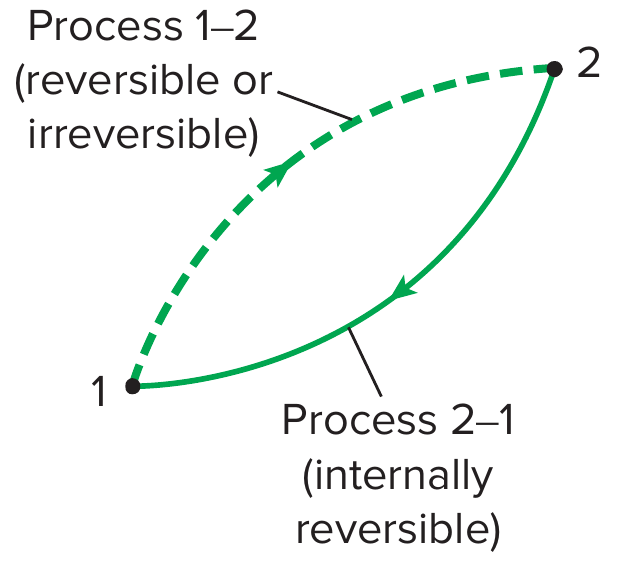
\includegraphics[scale=0.35]{Heat_Engine_Clausius_Inequality.png}
  \caption{Heat Engines and the Clausius Inequality}
  \label{fig:Heat_Engine_Clausius_Inequality}
\end{figure}

Namely, the thing we can say is:
\begin{align*}
  \int\limits_{1}^{2} \frac{d \Heat}{\Temp} + \int\limits_{2}^{1} \frac{d \Heat}{\Temp} &\leq 0 \\
  \int\limits_{1}^{2} \Entropy + \int\limits_{2}^{1} \Entropy &\leq 0 \\
  (\Entropy_{1} - \Entropy_{2}) + \int\limits_{2}^{1} \Entropy &\leq 0 \\
  \Entropy_{2} - \Entropy_{1} &\geq \int\limits_{2}^{1} \frac{d \Heat}{\Temp}
\end{align*}

This last point is actually quite important and is restated here.
\begin{equation}\label{eq:Reversible_Process_Entropy_Lost}
  \Entropy_{2} - \Entropy_{1} \geq \int\limits_{2}^{1} \frac{d \Heat}{\Temp}
\end{equation}

\Cref{eq:Reversible_Process_Entropy_Lost} states that for an \nameref{def:Irreversible_Process}, \nameref{def:Work} is lost \textbf{forever}.
\begin{itemize}[noitemsep]
\item For \nameref{def:Irreversible_Process}es, $\Entropy$ \textbf{always} increases.
\item For \nameref{def:Reversible_Process}es, $\Change{\Entropy} = 0$.
\end{itemize}

%%% Local Variables:
%%% mode: latex
%%% TeX-master: "../../MMAE_320-Thermo-Reference_Sheet"
%%% End:
